\section{Congestion Control in Internet networks}
\subsection{Problem description}
A key characteristic of IP networks is their packet switching mechanism that allows a significant increase in the efficiency of bandwidth utilization. This efficiency is explained by the fact that multiple communications could take place over the same physical resource. However, this scheme rises the important question of how the capacity should be shared. And Internet discovered this in the hard way; during the mid 80' a serial of network crashes took place: high packet delay, high loss rate and  low  goodputs are the characteristics of the communications taking place then. These are now the symptoms of a network being over-utilized, and though these collapses had been baptised as Congestion Collapses \cite{RFC896}. 

As described in the RFC, the causes of this problems is that the offered load in the network is overpassing the network capacity resulting in full queues and so increase delay and more packets being drop. The same RFC state that the problem particularly occurs when TCP is the transport layer being used over IP. Rightly, TCP retransmission mechanism was really clumsy. Indeed, when the liable transport layer considers that a packet wasn't routed to destination it retransmits not only one but multiple packets. This means additional load over the already congested network and congestion getting worst. But even if this retransmission scheme was replaced, it is up to the end host to adapt their transmission rate to limit the congestion and enhance the overall network performance. This is what was achieved through the implementation of congestion avoidance algorithm proposed by Van Jacobson [Jacobson88] for TCP. The same report suggested also that the network performing congestion control might enhance further the global performance. Some of the techniques used by the network were introduced later in what is known today as Active Queue Management AQM.
\subsection{TCP and congestion control algorithm}
Transmission Control Protocol TCP is a transport layer protocol that provides a connection-oriented, reliable stream delivery service over the connectionless unreliable IP network. As a transport protocol it provides a demultiplexing function that allows several process or flows at a single IP address to communicate concurrently. It provides also reliability by establishing a connection with the destination end host, so data is transferred and acknowledge in terms of byte streams enabling thus the possibility of retransmissions when the losses are detected either by the expiration of the acknowledgement timer or the reception of acknowledgement of previously acknowledged bytes (duplicate acks).

 \begin{figure}[h]
  \begin{center}
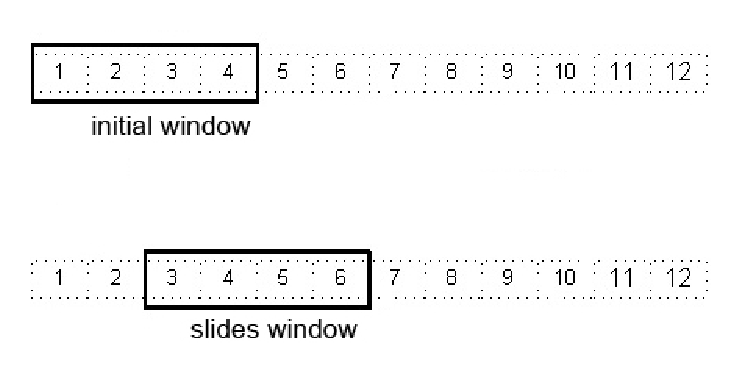
\epsfig{file=img/eps/CC1, width=4.5in}
\caption{
  The concept of sliding window.
    \label{fig:swnd}
}
 \end{center}
\end{figure}

To avoid bandwidth wastes that usually go with positive acknowledgement schemes, TCP use a sliding window algorithm that limits the number of segment a sender could transmit before receiving acknowledgements. Once the acknowledgement of the first packet arrives the window slides and a next packet could be sent. The number of packets that could be sent before receiving a first acknowledgement is called the window size(Figure\ref{swnd}). Thus, the transmission rate of a sender could be estimated in function of the window size as:
\begin{equation}
R_{Tx} = \frac{Window size}{RTT}
\end{equation}
where RTT is the Round Trip Time which is the necessary time for the packet to arrive to the receiver and that the acknowledgement to get back. This window side is variable and limited by the receiver advertisement window, that allow the receiver to specify the number of bytes that it could receive, and also the congestion window that is used by the sender to limit the transmission rate to control the congestion. A variety of congestion control algorithms exist depending on TCP implementation but they all have “Slow Start” and “Congestion Avoidance” in common. 

 \begin{figure}[h]
  \begin{center}
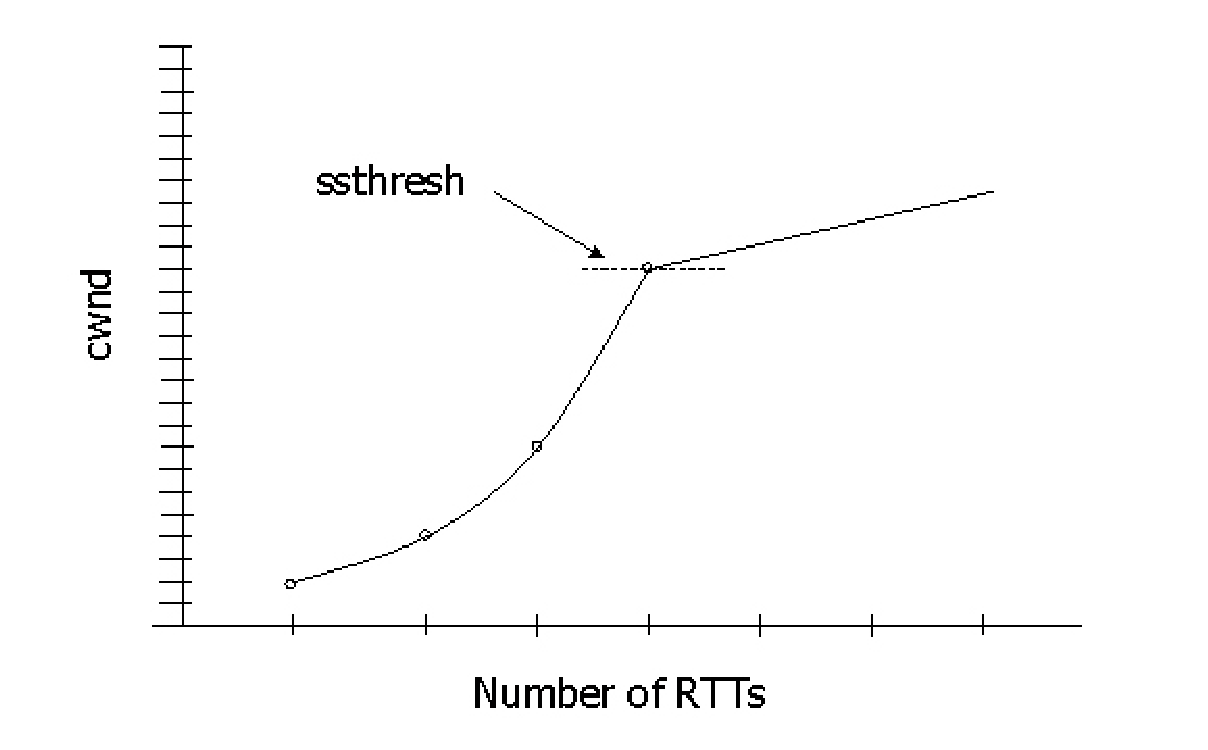
\epsfig{file=img/eps/CC2, width=4.5in}
\caption{
  Slow Start and Congestion Avoidance.
    \label{fig:SSCA}
}
 \end{center}
\end{figure}

So during the Slow Start phase the sender increase exponentially the congestion window {\it cwnd} until reaching the slow start threshold {\it ssthresh} then TCP sender enters the “Congestion Avoidance” phase where the cwnd is increased by 1 every time an acknowledgement is received.
TCP implementations differ on how to react to losses and how to identify them (Retransmission TimeOut (RTO) or duplicate acks): either by reducing the cwnd to 1 and enter again the "Slow Start", or to ssthresh in the case of “Fast Transmit” and TCP transmiters enter directly the phase of  “Congestion Avoidance”. {\it ssthresh} is reduced also and usually put to the half of the cwnd before that the congestion occurs. Thus this algorithm is designed as Additive Increase Multiplicative Decrease AIMD. 

\subsection{Active Queue Management}

An individual action from the end hosts toward the congestion presents some limitation. End hosts are only aware of the congestion when the packets start being dropped and they react simultaneously to the congestion causing thus a global synchronisation. RFC 2309 states that using some queue management techniques for congestion control will allow to decrease the number of dropped packets and avoid global synchronisation. 
RED or Random Early Discard is one of these scheme that permit to avoid oscillation and the global synchronisation by starting to discard packets randomly before the queue is completely full:

 \begin{figure}[h]
  \begin{center}
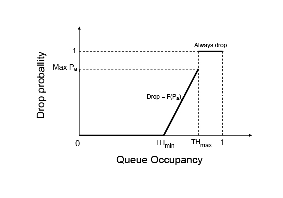
\epsfig{file=img/eps/CC3, width=4.5in}
\caption{
  Drop probabiliry in RED.
    \label{fig:RED}
}
 \end{center}
\end{figure}

The algorithm steps are the following:
1-If the queue size is smaller than $T_{min}$, packets are enqueued.
2-If queue size is larger than $T_{max}$ discard the packet.
3-If the queue size is between $T_{min}$ and $T_{max}$ packets are dropped according to a probability p.

The key to make the algorithm work is to well choose the algorithm parameters. Some of the consideration are to ensure a high utilization of the outgoing link and provision enough difference between $T_{min}$ and $T_{max}$ so the end hosts are informed and could react. Also differntial treatment could be applied by using different value of the discard probability p for different flow classes. 

{\bf Explicit Congestion Notification (ECN)}
\\RED could also be combined with ECN \cite {RFC 2481} another AQM technique that allows the network to explicitly inform the end user of the congestion instead of relying only on the the host detecting packet losses. The network feedback is passed to the end user through two unused bits in the IP TOS byte.  Thus 4 code points are available :\\

\begin{center}
\begin{tabular}{| l | c| } \hline 
00 & Non ECN-Capable Transport - Non-ECT \\ \hline 
10 & ECN Capable Transport - ECT(0) \\ \hline 
01 & ECN Capable Transport - ECT(1) \\ \hline 
11 & Congestion Encountered - CE  \\ \hline 
\end{tabular}
\\
\caption{
  ECN codepoint.
    \label{fig:ECN}
}
\end{center}

\\ECT(0) and ECT(1) indicates that the originator of the packet is ECN capable and in this case, if the packet has experienced congestion the router will mark the packet with CE code point. This is carried out in a similar scheme to RED and allows transport protocols and particularly TCP of being notified of congestion without having to experience loss. 
By marking packets instead of dropping them, ECN reduces the number of dropped packets. It also reduces the delay for the network layer to consider the packet as dropped and hence the delay of its reaction to the congestion. Finally, is in-band signalling mechanism and doesn't add additional traffic which is particularly harmful when the network is experiencing congestion.




